% Options for packages loaded elsewhere
\PassOptionsToPackage{unicode}{hyperref}
\PassOptionsToPackage{hyphens}{url}
%
\documentclass[
]{article}
\usepackage{amsmath,amssymb}
\usepackage{lmodern}
\usepackage{iftex}
\ifPDFTeX
  \usepackage[T1]{fontenc}
  \usepackage[utf8]{inputenc}
  \usepackage{textcomp} % provide euro and other symbols
\else % if luatex or xetex
  \usepackage{unicode-math}
  \defaultfontfeatures{Scale=MatchLowercase}
  \defaultfontfeatures[\rmfamily]{Ligatures=TeX,Scale=1}
\fi
% Use upquote if available, for straight quotes in verbatim environments
\IfFileExists{upquote.sty}{\usepackage{upquote}}{}
\IfFileExists{microtype.sty}{% use microtype if available
  \usepackage[]{microtype}
  \UseMicrotypeSet[protrusion]{basicmath} % disable protrusion for tt fonts
}{}
\makeatletter
\@ifundefined{KOMAClassName}{% if non-KOMA class
  \IfFileExists{parskip.sty}{%
    \usepackage{parskip}
  }{% else
    \setlength{\parindent}{0pt}
    \setlength{\parskip}{6pt plus 2pt minus 1pt}}
}{% if KOMA class
  \KOMAoptions{parskip=half}}
\makeatother
\usepackage{xcolor}
\usepackage[margin=1in]{geometry}
\usepackage{longtable,booktabs,array}
\usepackage{calc} % for calculating minipage widths
% Correct order of tables after \paragraph or \subparagraph
\usepackage{etoolbox}
\makeatletter
\patchcmd\longtable{\par}{\if@noskipsec\mbox{}\fi\par}{}{}
\makeatother
% Allow footnotes in longtable head/foot
\IfFileExists{footnotehyper.sty}{\usepackage{footnotehyper}}{\usepackage{footnote}}
\makesavenoteenv{longtable}
\usepackage{graphicx}
\makeatletter
\def\maxwidth{\ifdim\Gin@nat@width>\linewidth\linewidth\else\Gin@nat@width\fi}
\def\maxheight{\ifdim\Gin@nat@height>\textheight\textheight\else\Gin@nat@height\fi}
\makeatother
% Scale images if necessary, so that they will not overflow the page
% margins by default, and it is still possible to overwrite the defaults
% using explicit options in \includegraphics[width, height, ...]{}
\setkeys{Gin}{width=\maxwidth,height=\maxheight,keepaspectratio}
% Set default figure placement to htbp
\makeatletter
\def\fps@figure{htbp}
\makeatother
\setlength{\emergencystretch}{3em} % prevent overfull lines
\providecommand{\tightlist}{%
  \setlength{\itemsep}{0pt}\setlength{\parskip}{0pt}}
\setcounter{secnumdepth}{-\maxdimen} % remove section numbering
\usepackage{xcolor}
\definecolor{aliceblue}{HTML}{F0F8FF}
\definecolor{antiquewhite}{HTML}{FAEBD7}
\definecolor{aqua}{HTML}{00FFFF}
\definecolor{aquamarine}{HTML}{7FFFD4}
\definecolor{azure}{HTML}{F0FFFF}
\definecolor{beige}{HTML}{F5F5DC}
\definecolor{bisque}{HTML}{FFE4C4}
\definecolor{black}{HTML}{000000}
\definecolor{blanchedalmond}{HTML}{FFEBCD}
\definecolor{blue}{HTML}{0000FF}
\definecolor{blueviolet}{HTML}{8A2BE2}
\definecolor{brown}{HTML}{A52A2A}
\definecolor{burlywood}{HTML}{DEB887}
\definecolor{cadetblue}{HTML}{5F9EA0}
\definecolor{chartreuse}{HTML}{7FFF00}
\definecolor{chocolate}{HTML}{D2691E}
\definecolor{coral}{HTML}{FF7F50}
\definecolor{cornflowerblue}{HTML}{6495ED}
\definecolor{cornsilk}{HTML}{FFF8DC}
\definecolor{crimson}{HTML}{DC143C}
\definecolor{cyan}{HTML}{00FFFF}
\definecolor{darkblue}{HTML}{00008B}
\definecolor{darkcyan}{HTML}{008B8B}
\definecolor{darkgoldenrod}{HTML}{B8860B}
\definecolor{darkgray}{HTML}{A9A9A9}
\definecolor{darkgreen}{HTML}{006400}
\definecolor{darkgrey}{HTML}{A9A9A9}
\definecolor{darkkhaki}{HTML}{BDB76B}
\definecolor{darkmagenta}{HTML}{8B008B}
\definecolor{darkolivegreen}{HTML}{556B2F}
\definecolor{darkorange}{HTML}{FF8C00}
\definecolor{darkorchid}{HTML}{9932CC}
\definecolor{darkred}{HTML}{8B0000}
\definecolor{darksalmon}{HTML}{E9967A}
\definecolor{darkseagreen}{HTML}{8FBC8F}
\definecolor{darkslateblue}{HTML}{483D8B}
\definecolor{darkslategray}{HTML}{2F4F4F}
\definecolor{darkslategrey}{HTML}{2F4F4F}
\definecolor{darkturquoise}{HTML}{00CED1}
\definecolor{darkviolet}{HTML}{9400D3}
\definecolor{deeppink}{HTML}{FF1493}
\definecolor{deepskyblue}{HTML}{00BFFF}
\definecolor{dimgray}{HTML}{696969}
\definecolor{dimgrey}{HTML}{696969}
\definecolor{dodgerblue}{HTML}{1E90FF}
\definecolor{firebrick}{HTML}{B22222}
\definecolor{floralwhite}{HTML}{FFFAF0}
\definecolor{forestgreen}{HTML}{228B22}
\definecolor{fuchsia}{HTML}{FF00FF}
\definecolor{gainsboro}{HTML}{DCDCDC}
\definecolor{ghostwhite}{HTML}{F8F8FF}
\definecolor{gold}{HTML}{FFD700}
\definecolor{goldenrod}{HTML}{DAA520}
\definecolor{gray}{HTML}{808080}
\definecolor{green}{HTML}{008000}
\definecolor{greenyellow}{HTML}{ADFF2F}
\definecolor{grey}{HTML}{808080}
\definecolor{honeydew}{HTML}{F0FFF0}
\definecolor{hotpink}{HTML}{FF69B4}
\definecolor{indianred}{HTML}{CD5C5C}
\definecolor{indigo}{HTML}{4B0082}
\definecolor{ivory}{HTML}{FFFFF0}
\definecolor{khaki}{HTML}{F0E68C}
\definecolor{lavender}{HTML}{E6E6FA}
\definecolor{lavenderblush}{HTML}{FFF0F5}
\definecolor{lawngreen}{HTML}{7CFC00}
\definecolor{lemonchiffon}{HTML}{FFFACD}
\definecolor{lightblue}{HTML}{ADD8E6}
\definecolor{lightcoral}{HTML}{F08080}
\definecolor{lightcyan}{HTML}{E0FFFF}
\definecolor{lightgoldenrodyellow}{HTML}{FAFAD2}
\definecolor{lightgray}{HTML}{D3D3D3}
\definecolor{lightgreen}{HTML}{90EE90}
\definecolor{lightgrey}{HTML}{D3D3D3}
\definecolor{lightpink}{HTML}{FFB6C1}
\definecolor{lightsalmon}{HTML}{FFA07A}
\definecolor{lightseagreen}{HTML}{20B2AA}
\definecolor{lightskyblue}{HTML}{87CEFA}
\definecolor{lightslategray}{HTML}{778899}
\definecolor{lightslategrey}{HTML}{778899}
\definecolor{lightsteelblue}{HTML}{B0C4DE}
\definecolor{lightyellow}{HTML}{FFFFE0}
\definecolor{lime}{HTML}{00FF00}
\definecolor{limegreen}{HTML}{32CD32}
\definecolor{linen}{HTML}{FAF0E6}
\definecolor{magenta}{HTML}{FF00FF}
\definecolor{maroon}{HTML}{800000}
\definecolor{mediumaquamarine}{HTML}{66CDAA}
\definecolor{mediumblue}{HTML}{0000CD}
\definecolor{mediumorchid}{HTML}{BA55D3}
\definecolor{mediumpurple}{HTML}{9370DB}
\definecolor{mediumseagreen}{HTML}{3CB371}
\definecolor{mediumslateblue}{HTML}{7B68EE}
\definecolor{mediumspringgreen}{HTML}{00FA9A}
\definecolor{mediumturquoise}{HTML}{48D1CC}
\definecolor{mediumvioletred}{HTML}{C71585}
\definecolor{midnightblue}{HTML}{191970}
\definecolor{mintcream}{HTML}{F5FFFA}
\definecolor{mistyrose}{HTML}{FFE4E1}
\definecolor{moccasin}{HTML}{FFE4B5}
\definecolor{navajowhite}{HTML}{FFDEAD}
\definecolor{navy}{HTML}{000080}
\definecolor{oldlace}{HTML}{FDF5E6}
\definecolor{olive}{HTML}{808000}
\definecolor{olivedrab}{HTML}{6B8E23}
\definecolor{orange}{HTML}{FFA500}
\definecolor{orangered}{HTML}{FF4500}
\definecolor{orchid}{HTML}{DA70D6}
\definecolor{palegoldenrod}{HTML}{EEE8AA}
\definecolor{palegreen}{HTML}{98FB98}
\definecolor{paleturquoise}{HTML}{AFEEEE}
\definecolor{palevioletred}{HTML}{DB7093}
\definecolor{papayawhip}{HTML}{FFEFD5}
\definecolor{peachpuff}{HTML}{FFDAB9}
\definecolor{peru}{HTML}{CD853F}
\definecolor{pink}{HTML}{FFC0CB}
\definecolor{plum}{HTML}{DDA0DD}
\definecolor{powderblue}{HTML}{B0E0E6}
\definecolor{purple}{HTML}{800080}
\definecolor{red}{HTML}{FF0000}
\definecolor{rosybrown}{HTML}{BC8F8F}
\definecolor{royalblue}{HTML}{4169E1}
\definecolor{saddlebrown}{HTML}{8B4513}
\definecolor{salmon}{HTML}{FA8072}
\definecolor{sandybrown}{HTML}{F4A460}
\definecolor{seagreen}{HTML}{2E8B57}
\definecolor{seashell}{HTML}{FFF5EE}
\definecolor{sienna}{HTML}{A0522D}
\definecolor{silver}{HTML}{C0C0C0}
\definecolor{skyblue}{HTML}{87CEEB}
\definecolor{slateblue}{HTML}{6A5ACD}
\definecolor{slategray}{HTML}{708090}
\definecolor{slategrey}{HTML}{708090}
\definecolor{snow}{HTML}{FFFAFA}
\definecolor{springgreen}{HTML}{00FF7F}
\definecolor{steelblue}{HTML}{4682B4}
\definecolor{tan}{HTML}{D2B48C}
\definecolor{teal}{HTML}{008080}
\definecolor{thistle}{HTML}{D8BFD8}
\definecolor{tomato}{HTML}{FF6347}
\definecolor{turquoise}{HTML}{40E0D0}
\definecolor{violet}{HTML}{EE82EE}
\definecolor{wheat}{HTML}{F5DEB3}
\definecolor{white}{HTML}{FFFFFF}
\definecolor{whitesmoke}{HTML}{F5F5F5}
\definecolor{yellow}{HTML}{FFFF00}
\definecolor{yellowgreen}{HTML}{9ACD32}
\usepackage[most]{tcolorbox}

\usepackage{ifthen}
\provideboolean{admonitiontwoside}
\makeatletter%
\if@twoside%
\setboolean{admonitiontwoside}{true}
\else%
\setboolean{admonitiontwoside}{false}
\fi%
\makeatother%

\newenvironment{env-287ad2fb-bfc1-45fb-bc48-4c8f92527d7f}
{
    \savenotes\tcolorbox[blanker,breakable,left=5pt,borderline west={2pt}{-4pt}{firebrick}]
}
{
    \endtcolorbox\spewnotes
}
                

\newenvironment{env-09c22fe6-da77-4ae9-aa04-0de4f43f634a}
{
    \savenotes\tcolorbox[blanker,breakable,left=5pt,borderline west={2pt}{-4pt}{blue}]
}
{
    \endtcolorbox\spewnotes
}
                

\newenvironment{env-12fb5320-b8eb-47b6-8035-097e16242c42}
{
    \savenotes\tcolorbox[blanker,breakable,left=5pt,borderline west={2pt}{-4pt}{green}]
}
{
    \endtcolorbox\spewnotes
}
                

\newenvironment{env-351c71b8-ea6c-4dac-91c8-158f18380bf9}
{
    \savenotes\tcolorbox[blanker,breakable,left=5pt,borderline west={2pt}{-4pt}{aquamarine}]
}
{
    \endtcolorbox\spewnotes
}
                

\newenvironment{env-ab7dd5c8-11e4-4346-a2fa-55ec30fa26bb}
{
    \savenotes\tcolorbox[blanker,breakable,left=5pt,borderline west={2pt}{-4pt}{orange}]
}
{
    \endtcolorbox\spewnotes
}
                

\newenvironment{env-1af8abee-bd1a-4caf-83a0-2bb0e8d776aa}
{
    \savenotes\tcolorbox[blanker,breakable,left=5pt,borderline west={2pt}{-4pt}{blue}]
}
{
    \endtcolorbox\spewnotes
}
                

\newenvironment{env-b20d3313-6f31-4d49-96f7-b40d8676adb1}
{
    \savenotes\tcolorbox[blanker,breakable,left=5pt,borderline west={2pt}{-4pt}{yellow}]
}
{
    \endtcolorbox\spewnotes
}
                

\newenvironment{env-68e77820-1caa-45d1-9905-cf4d97c6beef}
{
    \savenotes\tcolorbox[blanker,breakable,left=5pt,borderline west={2pt}{-4pt}{darkred}]
}
{
    \endtcolorbox\spewnotes
}
                

\newenvironment{env-52a3b9de-376a-45de-b8df-e79f5b41a55c}
{
    \savenotes\tcolorbox[blanker,breakable,left=5pt,borderline west={2pt}{-4pt}{pink}]
}
{
    \endtcolorbox\spewnotes
}
                

\newenvironment{env-931ddf01-db8c-48cb-afe9-9ca0344de2f5}
{
    \savenotes\tcolorbox[blanker,breakable,left=5pt,borderline west={2pt}{-4pt}{cyan}]
}
{
    \endtcolorbox\spewnotes
}
                

\newenvironment{env-f80732d9-c652-4178-a300-08d2f6025262}
{
    \savenotes\tcolorbox[blanker,breakable,left=5pt,borderline west={2pt}{-4pt}{cyan}]
}
{
    \endtcolorbox\spewnotes
}
                

\newenvironment{env-bae5b384-a711-42f3-a8c9-6a85f243ef58}
{
    \savenotes\tcolorbox[blanker,breakable,left=5pt,borderline west={2pt}{-4pt}{purple}]
}
{
    \endtcolorbox\spewnotes
}
                

\newenvironment{env-b3a445e3-51cd-4523-adc6-b077ccebfe19}
{
    \savenotes\tcolorbox[blanker,breakable,left=5pt,borderline west={2pt}{-4pt}{darksalmon}]
}
{
    \endtcolorbox\spewnotes
}
                

\newenvironment{env-0cbdd535-e651-4c17-8f3a-ff3377c34628}
{
    \savenotes\tcolorbox[blanker,breakable,left=5pt,borderline west={2pt}{-4pt}{gray}]
}
{
    \endtcolorbox\spewnotes
}
                
\ifLuaTeX
  \usepackage{selnolig}  % disable illegal ligatures
\fi
\IfFileExists{bookmark.sty}{\usepackage{bookmark}}{\usepackage{hyperref}}
\IfFileExists{xurl.sty}{\usepackage{xurl}}{} % add URL line breaks if available
\urlstyle{same} % disable monospaced font for URLs
\hypersetup{
  pdftitle={Company Decision-making},
  hidelinks,
  pdfcreator={LaTeX via pandoc}}

\title{Company Decision-making}
\author{}
\date{}

\begin{document}
\maketitle

{
\setcounter{tocdepth}{3}
\tableofcontents
}
\hypertarget{decision-making}{%
\section{Decision-making}\label{decision-making}}

There are certain decisions which shareholders are required to take:

\begin{longtable}[]{@{}lll@{}}
\toprule()
Section & Decision & Resolution required \\
\midrule()
\endhead
s 190(1) & Approving a substantial property transaction (SPT) &
Ordinary \\
s 188(2) & Approving director's service contract for fixed term
{\(> 2\)} years & Ordinary \\
s 217(1) & Approving compensation to director for loss of office &
Ordinary \\
s 551(1) & Authorising directors to allot Shares & Ordinary \\
s 694(2) & Approving contract for share buyback & Ordinary \\
s 239(2) & Ratifying director's breach of duty & Ordinary \\
s 366(1) & Authorising political donations & Ordinary \\
s 168(1) & Removing a director against their will & Ordinary \\
s 510(2) & Removing company auditor & Ordinary \\
s 21(1) & Amending the company's Articles of Association & Special \\
ss 569(1), 570(1), 571(1) & Disapplying shareholders' pre-emption rights
& Special \\
s 716(1) & Approving payment for share buyback out of capital &
Special \\
s 97(1)(a) & Deciding to register company as public & Special \\
s 77(1) & Changing company name (provided no other procedure in
articles) & Special \\
MA 4(1) & Direct the board of directors how to act & Special \\
s 84(1)(b) IA 1986 & Liquidation \textgreater{} Members' Voluntary
Liquidation & Special \\
\bottomrule()
\end{longtable}

Some take effect immediately, others merely give permission for the
transaction to proceed. So some decisions require shareholders, others
require directors, others require both. A private company with {\(> 1\)}
shareholders can take shareholder decisions in two ways:

\begin{enumerate}
\tightlist
\item
  By passing a resolution at a shareholders' meeting
\item
  Shareholders' written resolution.
\end{enumerate}

\hypertarget{directors-decision-making}{%
\section{Directors' Decision-making}\label{directors-decision-making}}

Directors generally take decisions collectively as a board (except where
delegated). The board can take decisions at a board meeting or by
written resolution.

\hypertarget{sole-director}{%
\subsection{Sole Director}\label{sole-director}}

\begin{itemize}
\tightlist
\item
  A company can have just one director (s 154).
\item
  MA 7(2) of the model articles for private companies allows a sole
  director to take decisions however the director wishes.
\item
  A sole director must still keep a written record of decisions taken
  (minutes) for 10 years (s 248(2)).
\item
  A sole director does not have to make a declaration of interest. Where
  a company which should have more than one director currently only has
  a sole director, the director must make any necessary declarations of
  interests in writing (s 186).
\end{itemize}

\hypertarget{board-meeting}{%
\subsection{Board Meeting}\label{board-meeting}}

\hypertarget{calling-meeting}{%
\subsubsection{Calling Meeting}\label{calling-meeting}}

\begin{env-12fb5320-b8eb-47b6-8035-097e16242c42}

MA 9(1)

(1) Any director may call a directors' meeting by giving notice of the
meeting to the directors or by authorising the company secretary (if
any) to give such notice.

(2) Notice of any directors' meeting must indicate---

\begin{itemize}
\tightlist
\item
  (a) its proposed date and time;
\item
  (b) where it is to take place; and
\item
  (c) if it is anticipated that directors participating in the meeting
  will not be in the same place, how it is proposed that they should
  communicate with each other during the meeting.
\end{itemize}

(3) Notice of a directors' meeting must be given to each director, but
need not be in writing.

(4) Notice of a directors' meeting need not be given to directors who
waive their entitlement to notice of that meeting, by giving notice to
that effect to the company not more than 7 days after the date on which
the meeting is held. Where such notice is given after the meeting has
been held, that does not affect the validity of the meeting, or of any
business conducted at it.

\end{env-12fb5320-b8eb-47b6-8035-097e16242c42}

\hypertarget{notice}{%
\subsubsection{Notice}\label{notice}}

Reasonable notice of a board meeting is necessary ((Re Homer District
Consolidated Gold Mines, ex parte Smith (1888) 39 Ch D 546), and this is
whatever notice it is usual for the directors to give (Brown v La
Trinidad (1887) 37 Ch. D. 1). Therefore, if all the directors are in the
same building, the meeting could be called almost immediately, if such
notice is customary for the directors.

There is no need to specify the business of the meeting (La Compagnie de
Mayville v Whitley {[}1896{]} 1 Ch 788 (CA)).

If notice is not given to a director, they can demand another meeting be
held within a reasonable time (Brown v La Trinidad (1887) 37 Ch. D. 1).

\hypertarget{quorum}{%
\subsubsection{Quorum}\label{quorum}}

\begin{env-b20d3313-6f31-4d49-96f7-b40d8676adb1}

Quorum

The minimum number of directors who are required by the company's
articles to be present for valid decisions to be taken at that meeting.

\end{env-b20d3313-6f31-4d49-96f7-b40d8676adb1}

\begin{env-12fb5320-b8eb-47b6-8035-097e16242c42}

\href{https://www.gov.uk/government/publications/model-articles-for-private-companies-limited-by-shares/model-articles-for-private-companies-limited-by-shares\#quorum}{Art
11 MA}

(1) At a directors' meeting, unless a quorum is participating, no
proposal is to be voted on, except a proposal to call another meeting.

(2) The quorum for directors' meetings may be fixed from time to time by
a decision of the directors, but it must never be less than two, and
unless otherwise fixed it is two.

(3) If the total number of directors for the time being is less than the
quorum required, the directors must not take any decision other than a
decision---

\begin{itemize}
\tightlist
\item
  (a) to appoint further directors, or
\item
  (b) to call a general meeting so as to enable the shareholders to
  appoint further directors.
\end{itemize}

\end{env-12fb5320-b8eb-47b6-8035-097e16242c42}

\begin{itemize}
\tightlist
\item
  Special articles can be adopted to change quorum rules.
\item
  There is no provision to allow for the appointment of alternates.
\item
  Not all directors necessarily count in the quorum, e.g., if a
  particular director has a personal interest in a transaction.
\end{itemize}

\begin{env-b20d3313-6f31-4d49-96f7-b40d8676adb1}

Quorate

A meeting at which the quorum is present.

\end{env-b20d3313-6f31-4d49-96f7-b40d8676adb1}

\hypertarget{director-interest-quorum}{%
\paragraph{Director Interest \& Quorum}\label{director-interest-quorum}}

\begin{env-12fb5320-b8eb-47b6-8035-097e16242c42}

MA 14

(1) If a proposed decision of the directors is concerned with an actual
or proposed transaction or arrangement with the company in which a
director is interested, that director is not to be counted as
participating in the decision-making process for quorum or voting
purposes.

(2) But if paragraph (3) applies, a director who is interested in an
actual or proposed transaction or arrangement with the company is to be
counted as participating in the decision-making process for quorum and
voting purposes.

(3) This paragraph applies when---

\begin{itemize}
\tightlist
\item
  (a) the company by ordinary resolution disapplies the provision of the
  articles which would otherwise prevent a director from being counted
  as participating in the decision-making process;
\item
  (b) the director's interest cannot reasonably be regarded as likely to
  give rise to a conflict of interest; or
\item
  (c) the director's conflict of interest arises from a permitted cause.
\end{itemize}

(4) For the purposes of this article, the following are permitted
causes---

\begin{itemize}
\tightlist
\item
  (a) a guarantee given, or to be given, by or to a director in respect
  of an obligation incurred by or on behalf of the company or any of its
  subsidiaries;
\item
  (b) subscription, or an agreement to subscribe, for shares or other
  securities of the company or any of its subsidiaries, or to
  underwrite, sub-underwrite, or guarantee subscription for any such
  shares or securities; and
\item
  (c) arrangements pursuant to which benefits are made available to
  employees and directors or former employees and directors of the
  company or any of its subsidiaries which do not provide special
  benefits for directors or former directors.
\end{itemize}

\end{env-12fb5320-b8eb-47b6-8035-097e16242c42}

\hypertarget{voting}{%
\paragraph{Voting}\label{voting}}

MA 7(1): each director has one vote at a board meeting, and all
resolutions maybe passed by majority vote. If there is an equal number
of votes for and against a resolution there is deadlock and the negative
view will prevail, which means that the resolution is defeated unless
the chairperson has a casting vote.

MA 10: voting can be flexible and take place by electronic means.

\hypertarget{chairperson}{%
\paragraph{Chairperson}\label{chairperson}}

\begin{itemize}
\tightlist
\item
  If there is any dispute over the ability of a particular director to
  vote/ count in the quorum on any issue, the chairperson must decide
  and their decision is final.
\item
  If there is deadlock, the chairperson (if appointed under Art 12 MA)
  has the casting vote (Art 13 MA).

  \begin{itemize}
  \tightlist
  \item
    MA also goes further and grant this casting vote to a director who
    chairs the meeting without formally being appointed as chairperson.
  \item
    MA 13(2) does exclude the casting vote, though, if the chairperson
    is prevented from voting or counting in the quorum under art 14.
  \item
    Often excluded in the articles.
  \end{itemize}
\end{itemize}

\hypertarget{administration}{%
\paragraph{Administration}\label{administration}}

\begin{itemize}
\tightlist
\item
  Minutes must be recorded for every board meeting and kept for 10
  years, otherwise an offence is committed by every officer of the
  company in default (CA 2006, s 248).
\item
  Minutes do not record verbatim what was said
\item
  s 1135(1) of the CA 2006 requires minutes to be kept in hard-copy or
  electronic form
\item
  MA 15: require minutes to be in written form.
\item
  The minutes are open to inspection by the directors (Conway v
  Petronius Clothing Co {[}1978{]} 1 WLR 72), but usually not by the
  shareholders (R v Mariquita and New Grenada Mining Company (1859) 1 El
  \& El 289).
\end{itemize}

\hypertarget{evidence-of-propriety}{%
\paragraph{Evidence of Propriety}\label{evidence-of-propriety}}

If the minutes of the meeting are signed by the chairperson, they are
evidence of the proceedings at that meeting (CA 2006, s 249(1)).

Unless the contrary is proved, where minutes are prepared in accordance
with s 248, the meeting is deemed duly held, all proceedings are deemed
to have taken place and all appointments are deemed validly made (s
249(1)).

\hypertarget{directors-written-resolutions}{%
\subsection{Directors' Written
Resolutions}\label{directors-written-resolutions}}

NON-EXAMINABLE: Allows directors to take decisions without having to
call and hold a board meeting. Permitted under MA 8(2).

\begin{env-12fb5320-b8eb-47b6-8035-097e16242c42}

MA 8(2)

(1) A decision of the directors is taken in accordance with this article
when all eligible directors indicate to each other by any means that
they share a common view on a matter.

(2) Such a decision may take the form of a resolution in writing, copies
of which have been signed by each eligible director or to which each
eligible director has otherwise indicated agreement in writing.

(3) References in this article to eligible directors are to directors
who would have been entitled to vote on the matter had it been proposed
as a resolution at a directors' meeting.

(4) A decision may not be taken in accordance with this article if the
eligible directors would not have formed a quorum at such a meeting.

\end{env-12fb5320-b8eb-47b6-8035-097e16242c42}

Notes:

\begin{itemize}
\tightlist
\item
  Only require all eligible directors to vote; so excludes e.g., those
  with a personal interest in a proposed transaction.
\item
  Allows for flexibility: copies of resolutions to do not need to be
  signed and decision of each of the directors does not need to be
  simultaneous.
\item
  MA 8 goes further and allows decisions by any means, including those
  which are not written. But it is always sensible to have a written
  record.
\end{itemize}

\hypertarget{keeping-a-record}{%
\subsubsection{Keeping a Record}\label{keeping-a-record}}

\begin{itemize}
\tightlist
\item
  No requirement to keep copies of written resolutions under CA -- s 248
  CA 2006 only applies to a board meeting.
\item
  MA 15 requires a written record of any written resolution to be kept
  for 10 years.
\end{itemize}

\hypertarget{general-meetings}{%
\section{General Meetings}\label{general-meetings}}

\hypertarget{who-can-call}{%
\subsection{Who Can Call}\label{who-can-call}}

\hypertarget{board-of-directors}{%
\subsubsection{Board of Directors}\label{board-of-directors}}

General Meetings are usually called by the board of directors
(\href{https://www.legislation.gov.uk/ukpga/2006/46/section/302}{s 302
CA 2006}) by passing a board resolution at a Board Meeting (Brown v La
Trinidad (1887) 37 Ch. D. 1). This is usually passed by a simple
majority vote of directors, or can be passed by a signed directors'
written resolution.

\begin{env-09c22fe6-da77-4ae9-aa04-0de4f43f634a}

Note

On a board resolution just to call a GM, MA stipulates that MA 14
restrictions on quorum and voting do not apply, since the board meeting
decision is seen as purely procedural.

\end{env-09c22fe6-da77-4ae9-aa04-0de4f43f634a}

The Board must give 14 clear days' notice of a General Meeting
(\href{https://www.legislation.gov.uk/ukpga/2006/46/section/307}{s
307(1) CA 2006} \&
\href{https://www.legislation.gov.uk/ukpga/2006/46/section/360}{s 360 CA
2006}). The exception is where the \textbf{short notice procedure} is
used (s 307(4)-(6)): if {\(\geq 90\%\)} of shareholders with voting
rights agree, the general meeting can take place on short notice, e.g.,
immediately after the board meeting (note this requisite percentage can
be changed between 90-95\% in the Articles).

The notice for a general meeting must be timely
(\href{https://www.legislation.gov.uk/ukpga/2006/46/section/307}{s 307
CA 2006}) and appropriate
(\href{https://www.legislation.gov.uk/ukpga/2006/46/section/311}{s 311
CA 2006}). The validity of resolutions passed at a general meeting
depends on proper notice being given.

\hypertarget{shareholders}{%
\subsubsection{Shareholders}\label{shareholders}}

Shareholders can themselves call a General Meeting s 303-305. If the
Board refuses to call a General Meeting, the shareholders have reserve
power to do so themselves.

\href{https://www.legislation.gov.uk/ukpga/2006/46/section/303}{s 303(1)
CA 2006}: shareholders together holding {\(\geq 5\%\)} of paid-up voting
share capital of the company can serve a request on the company
(\textbf{'s 303 request'}). Must state the general nature of the
business which shareholders wish to be dealt with at the General
Meeting.

Under \href{https://www.legislation.gov.uk/ukpga/2006/46/section/304}{s
304(1) CA 2006}: when directors receive s 303 request, must call for the
General Meeting within 21 days from the date of request, to be held on a
date not more than 28 days after the \textbf{date of notice} convening
General Meeting.

If directors fail to \textbf{call} a General Meeting, all the
shareholders who submitted the s 303 request, or any of them
representing {\(> 50\%\)} of the voting rights of those that submitted
the request, can themselves call a General Meeting (pursuant
to\href{https://www.legislation.gov.uk/ukpga/2006/46/section/305}{s 305
CA 2006}).

If they call it themselves, a General Meeting must be held within
\textbf{3 months} of the date that directors receive the initial
request.

\href{https://www.legislation.gov.uk/ukpga/2006/46/section/305}{s 305(6)
CA 2006}: if shareholders are forced to call the General Meeting
themselves, can recover reasonable expenses for doing so from the
company. Then the company can recoup monies from directors who should
have called the meeting in the first place.

MERMAID

\hypertarget{who-to-notify}{%
\subsubsection{Who to Notify}\label{who-to-notify}}

Notice must be given (s 310 CA 2006):

\begin{itemize}
\tightlist
\item
  To all shareholders
\item
  To every director
\item
  To the personal representative of a deceased member
\item
  To the trustee in bankruptcy of a bankrupt member.
\end{itemize}

Companies articles may make alternative provision (s 310(4)), e.g.,
common to exclude giving notice to shareholders living overseas. Must
also give notice to auditors (s 502(2)(a)).

\hypertarget{how-to-notify}{%
\subsubsection{How to Notify}\label{how-to-notify}}

Can be hard-copy (handed to shareholders, or posted to address appearing
on register--s 1143), electronically (Sch 5 part 3), via a website (sch
5 part 4), or some combination (s 308).

\hypertarget{content-of-notice}{%
\subsubsection{Content of Notice}\label{content-of-notice}}

Must include:

\begin{itemize}
\tightlist
\item
  Time, date and place of meeting (s 311(1))
\item
  General nature of business - subject to articles to the contrary (s
  311(2))
\item
  Statement of rights to appoint a proxy (s 325(1))
\item
  Full text of any special resolution to be proposed (s 283(6)(a)).\\
  - This cannot be subsequently amended at the GM (In the matter of Uniq
  PLC {[}2011{]} EWHC 749 (Ch))).\\
  - But can be corrected by an accompanying circular.
\end{itemize}

No similar requirement to include the full next of an ordinary
resolution, though this is common practice. Ordinary resolutions can be
amended at the GM, provided the change is not so radical as to make
notice of the meeting ineffective (Betts v MacNaghten {[}1910{]} 1 Ch
430).

If shareholders exercise their s 314(1) rights to have a statement
circulated before the GM, this must be circulated with notice of the GM
(s 315(1)).

\hypertarget{length-of-notice}{%
\subsubsection{Length of Notice}\label{length-of-notice}}

\begin{env-12fb5320-b8eb-47b6-8035-097e16242c42}

s 307 - Notice required of a GM

(1) A general meeting of a private company (other than an adjourned
meeting) must be called by notice of at least 14 days.

(2) A general meeting of a public company (other than an adjourned
meeting) must be called by notice of---

\begin{itemize}
\tightlist
\item
  (a) in the case of an annual general meeting, at least 21 days, and
\item
  (b) in any other case, at least 14 days.
\end{itemize}

(3) The company's articles may require a longer period of notice than
that specified in subsection (1) or (2).

(4) A general meeting may be called by shorter notice than that
otherwise required if shorter notice is agreed by the members.

(5) The shorter notice must be agreed to by a majority in number of the
members having a right to attend and vote at the meeting, being a
majority who---

\begin{itemize}
\tightlist
\item
  (a) together hold not less than the requisite percentage in nominal
  value of the shares giving a right to attend and vote at the meeting
  (excluding any shares in the company held as treasury shares), or
\item
  (b) in the case of a company not having a share capital, together
  represent not less than the requisite percentage of the total voting
  rights at that meeting of all the members.
\end{itemize}

(6) The requisite percentage is---

\begin{itemize}
\tightlist
\item
  (a) in the case of a private company, 90\% or such higher percentage
  (not exceeding 95\%) as may be specified in the company's articles;
\item
  (b) in the case of a public company, 95\%.
\end{itemize}

(7) Subsections (5) and (6) do not apply to an annual general meeting of
a public company (see instead section 337(2)).

\end{env-12fb5320-b8eb-47b6-8035-097e16242c42}

\begin{itemize}
\tightlist
\item
  14 clear days' notice (ss 307(1) \& 360).
\item
  Notice period usually includes weekends and bank holidays.
\item
  Where a company has unamended Table A articles, those articles may
  extend this notice period (s 307(3)).
\item
  The minimum notice period applicable to the GMs for public companies
  and traded companies is more complex.
\end{itemize}

\hypertarget{deemed-delivery}{%
\paragraph{Deemed Delivery}\label{deemed-delivery}}

\begin{env-0cbdd535-e651-4c17-8f3a-ff3377c34628}

Attention

In addition to the minimum 14 clear days' notice period, it is usually
necessary under s 1147 of the CA 2006 to add a further 48 hours before
the GM can be held, unless the company's articles state otherwise. This
is because s 1147 provides that a document (including a notice of a GM)
is deemed to have been received by the intended recipient 48 hours after
it was sent by post or electronically.

\end{env-0cbdd535-e651-4c17-8f3a-ff3377c34628}

\hypertarget{short-notice}{%
\subsubsection{Short Notice}\label{short-notice}}

It is possible for the shareholders of a company to agree to hold a GM
on short notice (CA 2006, s 307(4)), provided that:

\begin{enumerate}
\tightlist
\item
  a majority in number of the shareholders must agree to holding the
  meeting on short notice (CA 2006, s 307(5)); and
\item
  those shareholders must hold at least 90\% of the voting shares in the
  private company (s 307(5)(a) and (6)(a)). This 90\% threshold may be
  increased by the articles to 95\% (s 307(6)(a)), which applies to many
  companies formed before the CA 2006 came into force.
\end{enumerate}

There are circumstances for which short notice cannot be used, e.g., s
168 removal of a director.

\hypertarget{invalid-notice}{%
\subsubsection{Invalid Notice}\label{invalid-notice}}

\begin{itemize}
\tightlist
\item
  Notice must be given in the proper form to all those entitled to it:
  if not done, then any resolutions purportedly passed at the meeting
  may be invalid (s 301(a)).
\item
  A deliberate decision not to send a notice to a shareholder can also
  amount to a s 171(b) breach by a director for exercising their powers
  for an improper purpose.
\end{itemize}

But:

\begin{env-12fb5320-b8eb-47b6-8035-097e16242c42}

s 313 - Accidental failure to give notice of resolution or meeting

(1) Where a company gives notice of---

\begin{itemize}
\tightlist
\item
  (a) a general meeting, or
\item
  (b) a resolution intended to be moved at a general meeting,
\end{itemize}

any accidental failure to give notice to one or more persons shall be
disregarded for the purpose of determining whether notice of the meeting
or resolution (as the case may be) is duly given.

(2) Except in relation to notice given under---

\begin{itemize}
\tightlist
\item
  (a) section 304 (notice of meetings required by members),
\item
  (b) section 305 (notice of meetings called by members), or
\item
  (c) section 339 (notice of resolutions at AGMs proposed by members),
\end{itemize}

subsection (1) has effect subject to any provision of the company's
articles

\end{env-12fb5320-b8eb-47b6-8035-097e16242c42}

\hypertarget{quorum-1}{%
\subsection{Quorum}\label{quorum-1}}

\begin{itemize}
\tightlist
\item
  Subject to the company's articles, the quorum for a General Meeting is
  two shareholders
  (\href{https://www.legislation.gov.uk/ukpga/2006/46/section/318}{s
  318(2) CA 2006})
\item
  For single member companies, of course, the quorum is one (s 318(1)).
\item
  No business other than the appointment of the chairman of the meeting
  can be transacted at a general meeting if the persons attending do not
  constitute a quorum
  (\href{https://www.gov.uk/government/publications/model-articles-for-private-companies-limited-by-shares/model-articles-for-private-companies-limited-by-shares\#quorumgen}{MA
  38}).
\item
  The quorum of a company with more than one shareholder cannot normally
  be reduced to one, because generally one person cannot constitute a
  `meeting' (Sharp v Dawes (1876) 2 QBD 26 (CA)).
\item
  In exceptional circumstances, the court may reduce the quorum to one
  under s 306 (e.g., where a shareholder refuses to attend a GM so that
  no decisions can be taken (Re El Sombrero Ltd {[}1958{]} Ch 900)).
\item
  GMs must be quorate throughout the meeting.
\end{itemize}

\hypertarget{conflicts}{%
\subsubsection{Conflicts}\label{conflicts}}

\begin{itemize}
\tightlist
\item
  Generally, there is no restriction on shareholders who have a conflict
  of interest voting in a GM as, unlike directors, they are not
  fiduciaries (Pender v Lushington (1877) 6 ChD 70).
\item
  Exceptions: shareholders with a conflict cannot vote on:

  \begin{itemize}
  \tightlist
  \item
    An ordinary resolution to ratify a director's breach of duty (if
    that director is also a shareholder) (s239).
  \item
    A special resolution to approve a buy-back out of share capital
    (that shareholder's vote is ignored) (s695 and s717)
  \end{itemize}
\end{itemize}

Note that this can be amended by the Articles; Table A makes the
threshold 95\%.

\hypertarget{proxies}{%
\subsubsection{Proxies}\label{proxies}}

\begin{itemize}
\tightlist
\item
  Proxies can usually count as part of the quorum.
\item
  But there must be at least two people physically present in the room
  for there to be a `meeting' (Re Sanitary Carbon Co {[}1870{]} WN 233),
  so can't have a single shareholder + proxy.
\end{itemize}

\hypertarget{permitted-attendees}{%
\subsubsection{Permitted Attendees}\label{permitted-attendees}}

The following can attend, though cannot vote unless they are also
shareholders:

\begin{itemize}
\tightlist
\item
  Directors (MA 40(1))
\item
  Auditors (s 502(2))
\item
  Anybody granted permission by the chairman (MA 40(2)).
\end{itemize}

\hypertarget{chairperson-1}{%
\subsection{Chairperson}\label{chairperson-1}}

\begin{itemize}
\tightlist
\item
  The Chairman at a GM does \textbf{not} get a casting vote -- an
  ordinary resolution can only be passed with a ``simple majority''
  i.e., more than 50\% (s282).
\item
  Role is to preside over meetings and keep order.
\item
  The Chairman will usually be the same person who is the chairman at
  board meetings (MA 39 provides that unless a Chairman is specifically
  appointed, the Chairman of Board meetings will automatically be the
  Chairman at GMs.
\end{itemize}

\hypertarget{voting-1}{%
\subsection{Voting}\label{voting-1}}

\hypertarget{methods-of-voting}{%
\subsubsection{Methods of Voting}\label{methods-of-voting}}

Two methods for passing both ordinary resolutions (s 282) and special
resolutions (s 283):

\begin{enumerate}
\tightlist
\item
  Show of hands -- each shareholder gets one vote (s 284(2))
\item
  Poll vote -- each shareholder gets one vote \textbf{per share} (s
  284(3)).
\end{enumerate}

Under
\href{https://www.gov.uk/government/publications/model-articles-for-private-companies-limited-by-shares/model-articles-for-private-companies-limited-by-shares\#votinggen}{MA
42} a resolution put to the vote of a General Meeting must be decided on
a show of hands unless a poll is demanded in accordance with the
Articles.
\href{https://www.gov.uk/government/publications/model-articles-for-private-companies-limited-by-shares/model-articles-for-private-companies-limited-by-shares\#pollvotes}{MA
44} deals with the right to demand a poll vote as follows:

\begin{env-12fb5320-b8eb-47b6-8035-097e16242c42}

MA 44 - Poll votes

(1) A poll on a resolution may be demanded---

\begin{itemize}
\tightlist
\item
  (a) in advance of the general meeting where it is to be put to the
  vote, or
\item
  (b) at a general meeting, either before a show of hands on that
  resolution or immediately after the result of a show of hands on that
  resolution is declared.
\end{itemize}

(2) A poll may be demanded by---

\begin{itemize}
\tightlist
\item
  (a) the chairman of the meeting;
\item
  (b) the directors;
\item
  (c) two or more persons having the right to vote on the resolution; or
\item
  (d) a person or persons representing \textbf{not less than one tenth
  of the total voting rights} of all the shareholders having the right
  to vote on the resolution.
\end{itemize}

(3) A demand for a poll may be withdrawn if---

\begin{itemize}
\tightlist
\item
  (a) the poll has not yet been taken, and
\item
  (b) the chairman of the meeting consents to the withdrawal.
\end{itemize}

(4) Polls must be taken immediately and in such manner as the chairman
of the meeting directs.

\end{env-12fb5320-b8eb-47b6-8035-097e16242c42}

If the vote is a poll vote, it is taken in writing with one vote per
share, usually immediately (R v Chillington Iron Co (1825) 29 ChD 159);
but votes cast in advance of the meeting may also be included in a poll
vote, subject to the articles of the company (s 322A).

\hypertarget{excluding}{%
\subsubsection{Excluding}\label{excluding}}

This right cannot be excluded:
\href{https://www.legislation.gov.uk/ukpga/2006/46/section/321}{s 321(1)
CA 2006} states that a provision of a company's articles is void in so
far as it would have the effect of excluding the right to demand a poll
at a general meeting on any question other than

\begin{itemize}
\tightlist
\item
  the election of the chairman of meeting;
\item
  the adjournment of the meeting
\end{itemize}

\hypertarget{proxies-1}{%
\subsubsection{Proxies}\label{proxies-1}}

\begin{env-12fb5320-b8eb-47b6-8035-097e16242c42}

s 324 - Rights to appoint proxies

(1) A member of a company is entitled to appoint another person as his
proxy to exercise all or any of his rights to attend and to speak and
vote at a meeting of the company.

(2) In the case of a company having a share capital, a member may
appoint more than one proxy in relation to a meeting, provided that each
proxy is appointed to exercise the rights attached to a different share
or shares held by him, or (as the case may be) to a different £10, or
multiple of £10, of stock held by him.

\end{env-12fb5320-b8eb-47b6-8035-097e16242c42}

\begin{itemize}
\tightlist
\item
  Corporate shareholders must appoint a representative to attend GMs
  (\href{https://www.legislation.gov.uk/ukpga/2006/46/section/323}{s 323
  CA 2006}).
\item
  The proxy must vote in accordance with the wishes of the shareholder
  who appointed the proxy (s 322A).
\item
  If a member wants to send a proxy to a meeting rather than attend
  personally, they must formally appoint a person as their proxy by
  depositing notice in writing at the registered office (MA 45).
\item
  Every notice of a GM must inform the shareholders clearly of their
  right to appoint proxies under s 324 of the CA 2006 and under any
  wider rights in the articles (s 325).
\item
  If it is intended to terminate a proxy's authority, the company must
  have received notice of that intention before the start of the
  relevant GM (CA 2006, s 330).
\item
  If the articles specify more than 48 hours' notice then that provision
  is void under s 330(6).
\end{itemize}

\hypertarget{annual-general-meeting}{%
\subsection{Annual General Meeting}\label{annual-general-meeting}}

Under CA 2006, private limited companies do \textbf{not} have to hold an
AGM, though public companies still do
(\href{https://www.legislation.gov.uk/ukpga/2006/46/section/336}{s 336
CA 2006}).

AGM must be called by directors
(\href{https://www.legislation.gov.uk/ukpga/2006/46/section/302}{s 302
CA 2006}) on 21 clear days'\textsuperscript{{[}1{]}} notice (s 307(2), s
360(2)) within 6 months' of the financial year-end. See also Company
procedure.

At the AGM, directors present an annual report. Shareholders with voting
rights vote on current issues, such as appointments to the company's
board of directors, executive compensation, dividend payments and the
selection of auditors.

\hypertarget{agm}{%
\subsubsection{AGM}\label{agm}}

\begin{itemize}
\tightlist
\item
  No requirement for private companies to hold an AGM.
\item
  But CA 2006 does not prevent a company from requiring an AGM in its
  articles.
\item
  CA 1985 stipulated there must be AGM
\item
  s 336(1) CA 2006 requires a public company to hold an AGM every year,
  in the 6 months after its accounting reference date.
\end{itemize}

\hypertarget{gm}{%
\subsubsection{GM}\label{gm}}

\begin{itemize}
\tightlist
\item
  MA companies only hold GMs, not AGMs
\item
  Pre-CA 2006, GMs were known as Extraordinary General Meetings (EGMs);
  the term is still used.
\end{itemize}

\hypertarget{resolutions}{%
\subsection{Resolutions}\label{resolutions}}

3 types of resolutions:

\begin{enumerate}
\tightlist
\item
  Ordinary resolution

  \begin{enumerate}
  \tightlist
  \item
    Passed by a simple majority ({\(> 49\%\)} of votes cast are in
    favour) --
    \href{https://www.legislation.gov.uk/ukpga/2006/46/section/282}{s
    282(1) CA 2006}.
  \end{enumerate}
\item
  Special resolution

  \begin{enumerate}
  \tightlist
  \item
    Requires a majority of {\(\geq 75\%\)}
    (\href{https://www.legislation.gov.uk/ukpga/2006/46/section/283}{s
    283(1) CA 2006}).
  \end{enumerate}
\item
  Extraordinary resolution

  \begin{enumerate}
  \tightlist
  \item
    Not mentioned in CA 2006, but it was a form of decision provided by
    in CA 1985. The majority required is the same as for a special
    resolution.
  \end{enumerate}
\end{enumerate}

If CA 2006 does not specify type of resolution to be used, ordinary
resolution required, unless Articles say higher majority
(\href{https://www.legislation.gov.uk/ukpga/2006/46/section/281}{s
281(3) CA 2006}). Special resolutions required for decisions like
amending the articles
(\href{https://www.legislation.gov.uk/ukpga/2006/46/section/21}{s 21 CA
2006}).

Votes at General Meetings counted out of all shareholders present and
voting.

\hypertarget{amendments}{%
\subsubsection{Amendments}\label{amendments}}

Where CA 2006 or the articles specify that an ordinary resolution may be
used, it is open to the shareholders to change the articles to require a
special resolution to be used instead (s 282(5)). The two exceptions to
this are removal of a director against their will (s 168) and the
removal of the company's auditors (s 510).

\hypertarget{deadlock}{%
\subsubsection{Deadlock}\label{deadlock}}

Pre-CA 2006 companies may allow a chairperson a casting vote in breaking
a deadlocked ordinary resolution. In exercising the power in this case,
the chairperson should cast their vote as a fiduciary rather than as an
individual; in other words, for what is best for the company rather than
for their personal position. Under CA 2006 this is no longer permitted.

\hypertarget{interests}{%
\subsubsection{Interests}\label{interests}}

\hypertarget{shareholders-may-vote-in-their-own-interests}{%
\paragraph{Shareholders May Vote in Their Own
Interests}\label{shareholders-may-vote-in-their-own-interests}}

General principle: shareholders may vote in their own interests.
Shareholders are under no fiduciary duty to help the company and can
vote as they wish, regardless of whether the vote will be in the best
interests of the company (Pender v Lushington (1877) 6 ChD 70).

Shareholders who are also directors can ignore Fiduciary duties when
voting in their capacity as shareholders ({[}North-West Transportation
Co Ltd v Beatty (1887) 12 App Cas 589{]}).

But shareholders must act in bona fides way (Clemens v Clemens Bros
{[}1976{]} 2 All ER 268). The principle applies to shareholders who are
also directors, when voting in their capacity as shareholders (Northern
Counties Securities Ltd v Jackson \& Steeple Ltd {[}1974{]} 1 WLR 1133).

Shareholders may vote as they wish to remove a director, provided due
process has been followed (Citco Banking Corporation NV v Pusser's Ltd
{[}2007{]} UKPC 13).

In exceptional circumstances, the courts have made orders to restrain a
shareholder from exercising their vote in a way that was
\textbf{irrational} (Standard Chartered Bank Ltd v Walker {[}1992{]} 1
WLR 561).

\hypertarget{restrictions}{%
\paragraph{Restrictions}\label{restrictions}}

There are times when the votes of a particular shareholder are ignored:

\begin{itemize}
\tightlist
\item
  Votes by a director/ connected person on an ordinary resolution to
  ratify a directors' breach of duty (s 239(4))
\item
  Votes on shares to be bought back, when shareholders voting by
  ordinary resolution on a share buyback (s 695) or by special
  resolution on a buyback out of capital (s 717).
\end{itemize}

\hypertarget{amending-articles}{%
\subsubsection{Amending Articles}\label{amending-articles}}

When shareholders are voting on a decision to amend the articles, the
court will look at whether reasonable shareholders could have considered
that the amendment was for the benefit of the company.

Shareholders must vote to amend the articles in good faith (Allen v Gold
Reefs of West Africa {[}1900{]} 1 Ch 656) and not undermine substantive
rights of minority shareholders. If they do this, the court may hold the
amendment invalid.

Sidebottom v Kershaw, Leese \& Co Ltd {[}1920{]} 1 Ch 154 (Court of
Appeal): alteration held valid in the alteration of the company.

Citco Banking Corporation NV v Pusser's Ltd {[}2007{]} UKPC 13: creation
of new class of shares held reasonable.

\hypertarget{unanimous-agreement}{%
\subsection{Unanimous Agreement}\label{unanimous-agreement}}

Re Duomatic Ltd {[}1969{]} 2 Ch 365 established the principle that
informal resolutions agreed by all the shareholders outside a formal
meeting will be valid and binding.

Must have unqualified agreement of \textbf{all} the shareholders,
whether this is express or implied, verbal or by conduct (Schofield v
Schofield {[}2011{]} EWCA Civ 103).

However, this does not allow shareholders to take decisions which would
be unlawful under the CA 2006, and it may not be valid for certain
resolutions, such as those required to reduce a company's capital (Re
Barry Artist {[}1985{]} 1 WLR 1305), or to dismiss a director or the
company's auditors.

\hypertarget{shareholders-written-resolutions}{%
\section{Shareholders' Written
Resolutions}\label{shareholders-written-resolutions}}

Usually quicker and cheaper than calling a general meeting.

\hypertarget{when}{%
\subsection{When}\label{when}}

\begin{longtable}[]{@{}ll@{}}
\toprule()
Company types & Using shareholders' written resolutions \\
\midrule()
\endhead
Public companies & Never (s 281(2)) \\
Private companies & Always, except for dismissal of director or company
auditor (s 288(2)), to allow the party to speak at a GM to defend
themselves. \\
\bottomrule()
\end{longtable}

\hypertarget{procedure}{%
\subsection{Procedure}\label{procedure}}

\begin{longtable}[]{@{}ll@{}}
\toprule()
Legislation & Rule \\
\midrule()
\endhead
\href{https://www.legislation.gov.uk/ukpga/2006/46/section/281}{s 281 CA
2006} & Only Private companies can pass shareholders resolution by way
of written resolution \\
\href{https://www.legislation.gov.uk/ukpga/2006/46/section/282}{s 282 CA
2006} & Written ordinary resolution can be passed by simple majority of
total voting rights \\
\href{https://www.legislation.gov.uk/ukpga/2006/46/section/283}{s 283 CA
2006} & Written special resolution can be passed by majority of members
with {\(\geq 75\%\)} of total voting rights \\
\href{https://www.legislation.gov.uk/ukpga/2006/46/section/284}{s 284 CA
2006} & Where company has a share capital, every member has one vote in
respect to each share held, during a written resolution \\
\href{https://www.legislation.gov.uk/ukpga/2006/46/section/288}{s 288 CA
2006} & Resolutions to remove director or auditor from office can't be
done by written resolution \\
\bottomrule()
\end{longtable}

\begin{itemize}
\tightlist
\item
  Normally, \textbf{board's responsibility} to initiate (s 291(1))
\item
  s 292: shareholders can also require circulation of written
  resolution:
\end{itemize}

\begin{env-12fb5320-b8eb-47b6-8035-097e16242c42}

s 292 - Members' power to require circulation of written resolution

(1) The members of a private company may require the company to
circulate a resolution that may properly be moved and is proposed to be
moved as a written resolution.

(2) Any resolution may properly be moved as a written resolution
unless---

\begin{itemize}
\tightlist
\item
  (a) it would, if passed, be ineffective (whether by reason of
  inconsistency with any enactment or the company's constitution or
  otherwise),
\item
  (b) it is defamatory of any person, or
\item
  (c) it is frivolous or vexatious.
\end{itemize}

(3) Where the members require a company to circulate a resolution they
may require the company to circulate with it a statement of not more
than 1,000 words on the subject matter of the resolution.

(4) A company is required to circulate the resolution and any
accompanying statement once it has received requests that it do so from
members representing not less than the requisite percentage of the total
voting rights of all members entitled to vote on the resolution.

(5) The ``requisite percentage'' is 5\% or such lower percentage as is
specified for this purpose in the company's articles.

(6) A request---\\
(a) may be in hard copy form or in electronic form,\\
(b) must identify the resolution and any accompanying statement, and\\
(c) must be authenticated by the person or persons making it.

\end{env-12fb5320-b8eb-47b6-8035-097e16242c42}

\hypertarget{circulation}{%
\subsection{Circulation}\label{circulation}}

\begin{itemize}
\tightlist
\item
  A written resolution proposed by the directors or the requisitioning
  shareholders must be circulated to all `eligible members' (ss 291(2)
  and 293(1) respectively) and to the auditors (s 502(1)).
\item
  Circulation can be hard copy, electronic or by website, though bear in
  mind requirements relating to electronic communication with
  shareholders (ss 298 \& 299).
\end{itemize}

\begin{env-b20d3313-6f31-4d49-96f7-b40d8676adb1}

Eligible member

A shareholder who would have been entitled to vote on the `circulation
date' of the written resolution (s 289(1)).

\end{env-b20d3313-6f31-4d49-96f7-b40d8676adb1}

\begin{env-b20d3313-6f31-4d49-96f7-b40d8676adb1}

Circulation date

The date on which a resolution is first sent to an eligible member (s
290).

\end{env-b20d3313-6f31-4d49-96f7-b40d8676adb1}

\hypertarget{agreement}{%
\subsection{Agreement}\label{agreement}}

A shareholder agrees to a written resolution when the company receives
an authenticated document from the member, identifying the resolution
and indicating agreement (s 296(1)). Note, this is pretty flexible.

\hypertarget{majority}{%
\subsubsection{Majority}\label{majority}}

\begin{longtable}[]{@{}ll@{}}
\toprule()
Ordinary resolution & Special resolution \\
\midrule()
\endhead
{\(> 50\%\)} of the total voting rights of all eligible members. &
{\(\geq 75\%\)} total voting rights of all eligible members. \\
\bottomrule()
\end{longtable}

Total voting rights are calculated on the basis of one vote per share,
subject to anything to the contrary in the articles.

\hypertarget{deadline}{%
\subsubsection{Deadline}\label{deadline}}

A proposed written resolution must be passed before the end of
\textbf{28 days} beginning on the circulation date or the period
specified in the articles if different, otherwise it will lapse (s
297(1)) and any agreement signified by an eligible member after this
date is ineffective (s 297(2)).

\hypertarget{single-member-companies}{%
\subsection{Single Member Companies}\label{single-member-companies}}

Can take decisions:

\begin{itemize}
\tightlist
\item
  By GM resolution (s 301)
\item
  By passing a written resolution
\item
  By taking an informal decision.
\end{itemize}

Important to keep proof of details of decisions which could have been
taken at a GM (s 357).

\hypertarget{post-decision-requirements}{%
\subsection{Post-decision
Requirements}\label{post-decision-requirements}}

\hypertarget{filing}{%
\subsubsection{Filing}\label{filing}}

Usually need to file a form, shareholder resolution or related document
after taking a decision.

\hypertarget{resolutions-1}{%
\paragraph{Resolutions}\label{resolutions-1}}

\begin{itemize}
\tightlist
\item
  ss 29 \& 30: all copies of special resolutions/ written resolutions/
  decisions taken by unanimous consent must be sent to Registrar of
  Companies.

  \begin{itemize}
  \tightlist
  \item
    Must be done within 15 days (s 30(1)),
  \item
    else an offence is committed (s 30(2)).
  \end{itemize}
\item
  Certain other resolutions must be sent to Companies House
\item
  s 355(1) of the CA 2006, a company must keep records of all
  resolutions passed otherwise than at a GM (e.g., written resolutions)

  \begin{itemize}
  \tightlist
  \item
    These records must be kept for a minimum of 10 years (s 355(2)) at
    the company's registered office or SAIL (s 358(1))
  \item
    otherwise an offence is committed by every officer in default (s
    355(3)).
  \end{itemize}
\end{itemize}

\hypertarget{forms}{%
\paragraph{Forms}\label{forms}}

There are various forms.

\hypertarget{documents}{%
\paragraph{Documents}\label{documents}}

For example, if a special resolution to amend the company's articles is
passed by the shareholders under s 21, a copy of the amended articles
must be filed at Companies House not later than 15 days after the
special resolution is passed (s 26(1)), along with the special
resolution.

In other cases, certain documents must be kept and made available for
inspection by shareholders and sometimes others, including

\begin{itemize}
\tightlist
\item
  a director's service contract (or written memorandum of its terms)
  under s 228 for at least one year after the end of the contract (ss
  228(3) and 229(1)).
\item
  A contract to buy back the company's shares must be kept for at least
  10 years and made available for inspection (s 702).
\item
  A company must also keep available for inspection a copy of any charge
  over the company's property (s 877).
\end{itemize}

\hypertarget{registers}{%
\paragraph{Registers}\label{registers}}

Main registers:

\begin{itemize}
\tightlist
\item
  Register of members
\item
  PSC register
\item
  Register of directors
\item
  Register of directors' residential addresses
\item
  Register of secretaries.
\end{itemize}

Under s 128B, private companies may elect not to keep their own
registers of members, PSCs, directors, directors' residential addresses
and secretaries. They can instead ensure that the necessary information
is filed and kept up-to-date on the central register for the company
held at Companies House in electronic form.

\hypertarget{minutes}{%
\paragraph{Minutes}\label{minutes}}

Minutes must be kept for all proceedings of GMs (CA 2006, s 355(1)(b))
for at least 10 years (s 355(2)) at the company's registered office or
SAIL (s 358(1)), otherwise an offence is committed by every officer of
the company in default.

The minutes are open to inspection free of charge by the shareholders (s
358(3)), who may request a copy subject to payment of a fee (s 358(4)).

If the minutes of the meeting are signed by the chairperson they are
evidence of the proceedings at that meeting (s 356(4)). Unless the
contrary is proved, where minutes are prepared the GM is deemed duly
held, all proceedings are deemed to have taken place and all
appointments are deemed validly made (s 356(5)).

\hypertarget{sail}{%
\paragraph{SAIL}\label{sail}}

Ordinarily records will be kept at the company's registered office.
Under the Companies (Company Records) Regulations 2008 (SI 2008/3006,
made under s 1136 CA 2006) the company may choose to keep these records
at a so-called `single alternative inspection location' (SAIL).

\hypertarget{joint-decision-making}{%
\subsection{Joint Decision-making}\label{joint-decision-making}}

For many decisions you need a board meeting sandwich. There is a choice
of whether to:

\begin{enumerate}
\tightlist
\item
  Leave the first meeting adjourned and then reconvene it
\item
  Hold board meetings.
\end{enumerate}

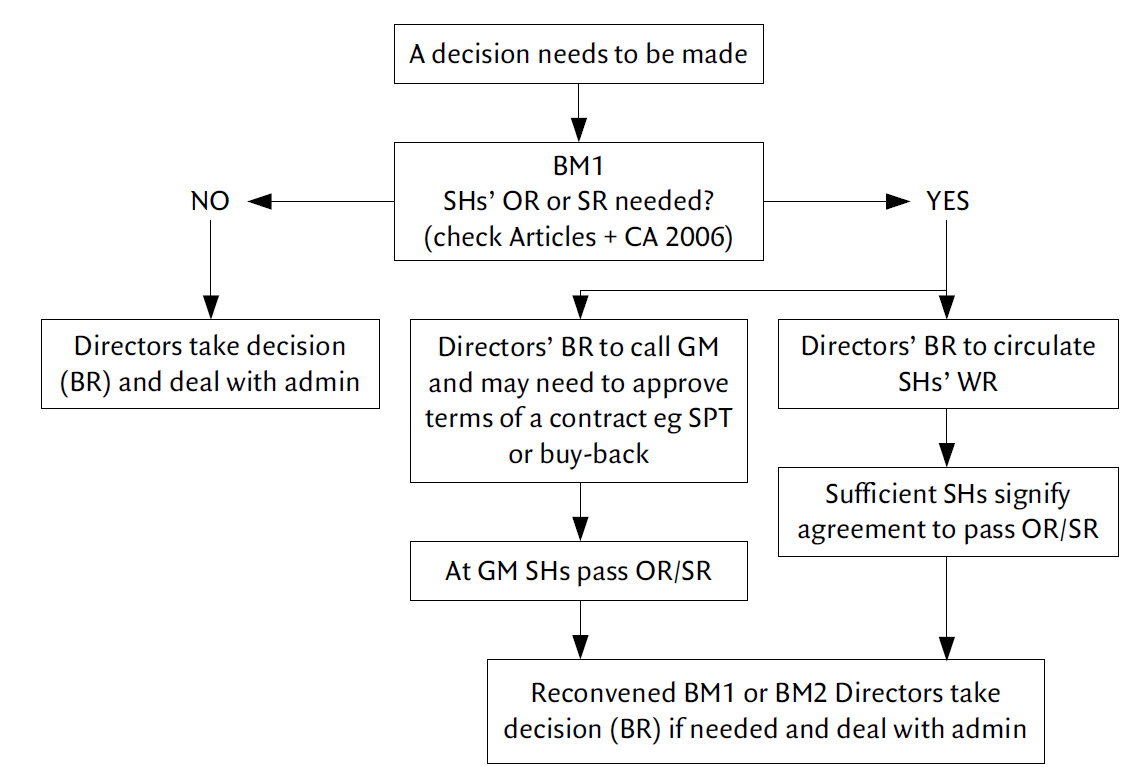
\includegraphics{C:/Users/shiva/Mega/LegalPracticeCourse/BM-GM-decision-flow.png}

\hypertarget{electronic-communication}{%
\subsection{Electronic Communication}\label{electronic-communication}}

Individual shareholders need to give their consent to be contacted by
the company by e-mail or other electronic means rather than by post (CA
2006, Sch 5, Part 3, para 6).

The shareholders may pass a resolution authorising the use of a company
website for communication, or the articles may so provide. If either is
the case, the individual shareholders are required to opt out of using
the website rather than to opt in (CA 2006, Sch 5, Part 4, para 10).

\begin{center}\rule{0.5\linewidth}{0.5pt}\end{center}

\begin{enumerate}
\tightlist
\item
  \protect\hypertarget{fn-1-af83d4929e2658fe}{}{``Clear days'' means the
  day the notice was given and the day of the meeting are discounted
  from calculation (s 360)}
\end{enumerate}

\end{document}
